\newpage
\section{Wärmelehre}

\subsection{Temperatureinheiten}				%Temperatureinheiten
\begin{table}[h!]
	\begin{tabular}{ | m{9cm} | m{9cm}  | }
		\hline
		Formeln & Einheiten \\ \hline
		\midrule
		%\begin{minipage}[t]{5cm}
		\begin{itemize}
			\item $^\circ\text{C}=\dfrac{^\circ\text{F}-32}{1.8}$
			\item $^\circ\text{F}=^\circ\text{C}*1.8+32$
			\item $^\circ\text{C}=K-273.15$
			\item $K=^\circ\text{C}+273.15$
			
		\end{itemize}
		%\end{minipage}
		&
		%\begin{minipage}{5cm}
		\begin{itemize}
			\item $^\circ\text{C}=$ Temperatur in Celsius
			\item $^\circ\text{F}=$ Temperatur in Fahrenheit
			\item $K=$ Temperatur in Celsius
		\end{itemize}
		%\end{minipage}
		\\ \hline
	\end{tabular}
\end{table}

\subsection{Molare Masse, Molmasse}				%Molare Masse, Molmasse
\begin{table}[h!]
	\begin{tabular}{ | m{9cm} | m{9cm}  | }
		\hline
		Formeln & Einheiten \\ \hline
		\midrule
		%\begin{minipage}[t]{5cm}
		\begin{itemize}
			\item $M=\dfrac{m}{n}=N_{A}*m_M$
			
			
		\end{itemize}
		%\end{minipage}
		&
		%\begin{minipage}{5cm}
		\begin{itemize}
			\item $m=[kg]$
			\item $n=[mol]$
			\item $M=[\frac{kg}{mol}]$
			\item $N_{A}=6.022*10^{23}$ $[\dfrac{1}{mol}] $
			\item $m_M=[kg]$
			
		\end{itemize}
		%\end{minipage}
		\\ \hline
	\end{tabular}
\end{table}

\subsection{Längen und Volumenänderung}				%Längen und Volumenänderung
\begin{table}[h!]
	\begin{tabular}{ | m{6cm} | m{8cm} | m{4cm} | }
		\hline
		Abbildung & Formeln & Einheiten \\ \hline
		\midrule
		\begin{minipage}{.3\textwidth}
			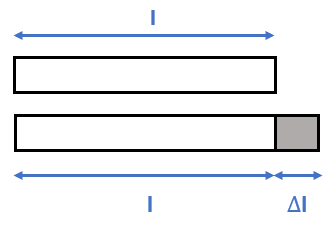
\includegraphics[width=6.0cm]{Figures/Deltal}
		\end{minipage}
		&
		%\begin{minipage}[t]{5cm}
		\begin{itemize}
			\item $\Delta l=\alpha*l*\Delta T$	
			\item $\Delta V=\gamma*V*\Delta T$	
			\item $\alpha,\gamma=Ausdehnungskoeffizienten$
			\item $\gamma=3*\alpha$ (Gilt bei isotopen Materialien)
			\item Isotop = In allen Richtungen gleiche Eigenschaften	
		\end{itemize}
		%\end{minipage}
		& 
		%\begin{minipage}{5cm}
		\begin{itemize}
			\item $\Delta l,l= [m]$
			\item $\Delta V,V=[m^3]$
			\item $\alpha,\gamma=[\frac{1}{K}]$	
			\item $\Delta T=[K]$
		\end{itemize}
		%\end{minipage}
		\\ \hline
	\end{tabular}
\end{table}

\subsection{Thermische Spannung, Hookesches Gesetz}				%Thermische Spannung, Hookesches Gesetz
\begin{table}[h!]
	\begin{tabular}{ | m{6cm} | m{8cm} | m{4cm} | }
		\hline
		Abbildung & Formeln & Einheiten \\ \hline
		\midrule
		\begin{minipage}{.3\textwidth}
			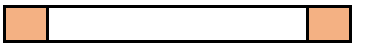
\includegraphics[width=6.0cm]{Figures/Spannung}
		\end{minipage}
		&
		%\begin{minipage}[t]{5cm}
		\begin{itemize}
			\item Ohne Behinderung: $\Delta l=\alpha*l*\Delta T$	
			\item Mit Behinderung: $\Delta l=0$	
			\item $\sigma=E*\dfrac{\Delta l}{l}$
			\item $\sigma=E*\alpha*\Delta T$
			\item E = Elastizitätsmodul
			\item $\sigma=$Thermische Spannung
		\end{itemize}
		%\end{minipage}
		& 
		%\begin{minipage}{5cm}
		\begin{itemize}
			\item $E= [\frac{N}{m^{2}}]=Pa$
			\item $\sigma=[\frac{N}{m^{2}}]=Pa$
			\item $\Delta l,l= [m]$
			\item $\Delta V=[m^3]$
			\item $\alpha=[\frac{1}{K}]$	
			\item $\Delta T=[K]$
		\end{itemize}
		%\end{minipage}
		\\ \hline
	\end{tabular}
\end{table}
\uline{\textbf{Thermodynamische Systeme}}

	$\Rightarrow$ offen = Austausch von Energie und Austausch von Material (z.B. Wärmetauscher, Kompressor, Gasturbine)\\
	$\Rightarrow$ geschlossen = Austausch von Energie und kein Austausch von Material (z.B. Heizkreislauf, Kühlschrank)\\
	$\Rightarrow$ abgeschlossen = kein Austausch von Energie und kein Austausch von Material (z.B. Ideale Thermosflasche)\\ 	
	$\Rightarrow$ adiabatisch = kein Wärmeaustausch, kein Materialaustausch, aber Energieaustausch (z.B. Kompressor)\\

\newpage

\subsection{Thermische Zustandsgleichung, ideales Gas}				%Thermische Zustandsgleichung
\begin{table}[h!]
	\begin{tabular}{ | m{9cm} | m{9cm}  | }
		\hline
		Formeln & Einheiten \\ \hline
		\midrule
		%\begin{minipage}[t]{5cm}
		\begin{itemize}
			\item $p*V=N*k*T$	
			\item $p*V=n*R*T$
			\item $p*V=\dfrac{m}{M}*R*T$
			\item $R=N_{A}*k$ 
			\item $n=\dfrac{m}{M}$
			\item R = Universelle Gaskonstante
			\item k = Boltzmann-Konstante
			\item $N_{A}$ = Avogadro-Zahl
			\item {\color{red}1 atü = $98066.5$ $ [Pa]$}
			\item {\color{red}1 Torr = $133.322$ $ [Pa] = 1[mm]*g*\rho_{Hg}$}
		\end{itemize}
		%\end{minipage}
		&
		%\begin{minipage}{5cm}
		\begin{itemize}
			\item $p= [\frac{N}{m^{2}}]=Pa$
			\item $V=[m^3]$
			\item $N=[1]=$ Anzahl Moleküle
			\item $n=[1]=$ Anzahl Mole
			\item $M=[\frac{kg}{mol}]=$ Molare Masse
			\item $T=[K]$
			\item $k=1.381*10^{-23}$ $[\frac{J}{K}]$
			\item $R=8.314$ $[ \frac{J}{mol*K} ]$
			\item $N_{A}=6.022*10^{23}$ $[\dfrac{1}{mol}] $
			\item $\rho_{Hg}=13595[\frac{kg}{m^3}]$
			\item $g=9.81[\frac{m}{s^2}]$
			
			
			
		\end{itemize}
		%\end{minipage}
		\\ \hline
	\end{tabular}
\end{table}

	 Ideales Gas $\Rightarrow$  \textbf{1.)} $(p*V=const)$            Teilchen sind Massepunkte \textbf{2b.)} Teilchen üben keine gegenseitigen Kräfte aus\\ 
	 Reales Gas $\Rightarrow$ \textbf{1.)}  Teilchen dehnen sich aus $\rightarrow$ Volumen ist jetzt: (V-b) \textbf{2.)} Teilchen wirken Kräfte aus $(p=p_{0}+\dfrac{a}{V^{2}})$\\
	 
	 \newpage
	

\subsection{Van der Waal'sche Zustandsgleichung, reale Gase}				%Van der Waal'sche Zustandsgleichung, reale Gase
\begin{table}[h!]
	\begin{tabular}{ | m{6cm} | m{6cm} | m{6cm} | }
		\hline
		Abbildung & Formeln & Einheiten \\ \hline
		\midrule
		\begin{minipage}{.3\textwidth}
			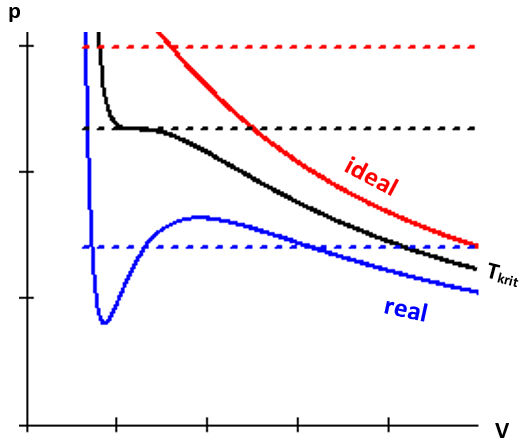
\includegraphics[width=6.0cm]{Figures/vanderwaal}
		\end{minipage}
		&
		%\begin{minipage}[t]{5cm}
		\begin{itemize}
			\item(allg.): $p=\dfrac{n*R*T}{V_{m}-b}-n^{2}*\dfrac{a}{V_{m}^{2}}$ 
			\item(1 mol): $p=\dfrac{R*T}{V_{m}-b}-n^{2}*\dfrac{a}{V_{m}^{2}}$
			\item $V=V_{m}*n$
			\item a = Kohäsionsdruck (materialabhängig)
			\item b = Kovolumen (materialabhängig)
		\end{itemize}
		%\end{minipage}
		& 
		%\begin{minipage}{5cm}
		\begin{itemize}
			\item $p= [\frac{N}{m^{2}}]=Pa$
			\item $V=[m^3]$
			\item $n=[1]=$ Anzahl Mole
			\item $V_{m}=[\frac{m^3}{mol}]=$ molares Volumen
			\item $T=[K]$
			\item $a=[\frac{10^{-3}*Pa*m^{6}}{mol^{2}}]$
			\item $b=[\frac{10^{-6}*m^{3}}{mol}]$
			
		\end{itemize}
		%\end{minipage}
		\\ \hline
	\end{tabular}
\end{table}

\subsection{Mittlere freie Weglänge}				%Mittlere freie Weglänge
\begin{table}[h!]
	\begin{tabular}{ | m{6cm} | m{7.5cm} | m{4.5cm} | }
		\hline
		Abbildung & Formeln & Einheiten \\ \hline
		\midrule
		\begin{minipage}{.3\textwidth}
			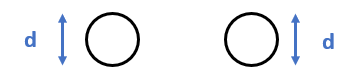
\includegraphics[width=6.0cm]{Figures/Weglaenge}
		\end{minipage}
		&
		%\begin{minipage}[t]{5cm}
		\begin{itemize}
			\item\={l} $ =\dfrac{1}{\sqrt{2}*n*\pi*d^{2}}=\dfrac{R*T}{\sqrt{2}*\pi*d^2*p*N_A}$ 
			\item $n=\dfrac{N}{V}=\dfrac{p*N_A}{R*T}$
			
		\end{itemize}
		%\end{minipage}
		& 
		%\begin{minipage}{5cm}
		\begin{itemize}
			\item\={l} $ =[m]$ 
			\item$n=\dfrac{Teilchen}{Volumen}=[\dfrac{1}{m^{3}}]$
			\item$d=[m]$
			\item $N=[1]$
			\item $V=[m^3]$
			\item $p=[Pa]$
			\item $T=[K]$
			\item $N_{A}=6.022*10^{23}$ $[\dfrac{1}{mol}]$
			\item $R=8.314$ $[ \frac{J}{mol*K} ]$
			
		\end{itemize}
		%\end{minipage}
		\\ \hline
	\end{tabular}
\end{table}

\newpage

\subsection{kinetische Gastheorie}				%kinetische Gastheorie
\begin{table}[h!]
	\begin{tabular}{ | m{6cm} | m{6cm} | m{6cm} | }
		\hline
		Abbildung & Formeln & Einheiten \\ \hline
		\midrule
		\begin{minipage}{.3\textwidth}
			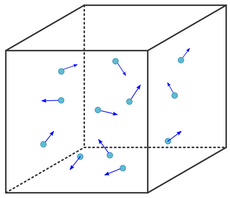
\includegraphics[width=6.0cm]{Figures/Gastheorie}
		\end{minipage}
		&
		%\begin{minipage}[t]{5cm}
		\begin{itemize}
			\item$p=\dfrac{F}{A}=\dfrac{1}{3}*\dfrac{_{N_{A}*v^{2}*m}}{V}$ 
			\item$E_{kin}=\dfrac{m*v^{2}}{2}=\dfrac{3}{2}*k*T$
			
		\end{itemize}
		%\end{minipage}
		& 
		%\begin{minipage}{5cm}
		\begin{itemize}
			\item $p= [\frac{N}{m^{2}}]=Pa$
			\item $F=[N]$
			\item $A=[m^2]$
			\item $V=[m^3]$
			\item $m=[kg]$
			\item $v=[m\frac{m}{s}]$
			\item $T=[K]$
			\item $k=1.381*10^{-23}$ $[\frac{J}{K}]$
			\item $N_{A}=6.022*10^{23}$ $[\dfrac{1}{mol}] $
			
		\end{itemize}
		%\end{minipage}
		\\ \hline
	\end{tabular}
\end{table}

\subsection{Thermodynamik}				%Thermodynamik
\begin{table}[h!]
	\begin{center}
	\begin{tabular}{ | m{10cm} | m{8cm}  | }
		\hline
		Formeln & Einheiten \\ \hline
		\midrule
		%\begin{minipage}[t]{5cm}
		\begin{itemize}
			\item Erster Hauptsatz der Thermodynamik: $dU=\delta W+\delta Q$ 	
			\item $\Delta Q=m*c*\Delta T$
			\item $m*c=C$
			\item $\Delta T=T_{2}-T_{1}\Rightarrow$ {\color{red} So, dass es positives $\Delta T$ gibt}
			\item $Q_{ab}=Q_{zu}$
			\item $Q_{s}=$ Schmelzwärme $= q_{s}*m$ 	
			\item $Q_{v}=$ Verdampfungswärme $= q_{v}*m$
			\item $q_{s}=$ spez. Schmelzwärme
			\item $q_{v}=$ spez. Verdampfungswärme 	
			\item $T_{M}=$ Mischtemparatur zweier Stoffe
			\item $T_{M}=\dfrac{m_{1}*c_{1}*T_{1}+m_{2}*c_{2}*T_{2}}{m_{1}*c_{1}+m_{2}*c_{2}}$
		\end{itemize}
		%\end{minipage}
		&
		%\begin{minipage}{5cm}
		\begin{itemize}
			\item $dU=$innere Energie$=[J]$
			\item $\delta W=$Arbeit$=[Ws]$
			\item $\delta Q,\Delta Q=$Wärme$=[J]$
			\item $m,m_{1},m_{2}=[kg]$
			\item $c,c_{1},c_{2}=$ spez. Wärmekapazität $=[\frac{J}{kg*K}]$
			\item $C=$ Wärmekapazität $=[\frac{J}{kg}]$
			\item $\Delta T,T_{1},T_{2},T_{M}=[K]$
			\item $c_{Wasser}=4182[\frac{J}{kg*K}]$
			\item $c_{Eis}=2060[\frac{J}{kg*K}]$
			\item $Q_{s},Q_{v}=[J]$
			\item $q_{s},q_{v}=[\frac{J}{kg}]$
			\item $q_{s,Eis}=333700[\frac{J}{kg}]$
			\item $q_{v,Wasser}=2257000[\frac{J}{kg}]$
		\end{itemize}
		%\end{minipage}
		\\ \hline
	\end{tabular}
\end{center}
\end{table}

	\textbf{Gründe für eine höhere Wärmekapazität:}\\
	1.) Anzahl Freiheitsgrade\\
	2.) Grössere Anzahl an Teilchen (kleinere Dichte)\\
	\textbf{Anomalie des Wassers:}\\
	Höchste Dichte bei 4 \textcelsius $\Rightarrow$ Volumenzunahme bei Erhöhung und Verminderung der Temperatur\\
	

\subsection{Wärmetransport}		%Wärmetransport
\begin{table}[h!]
	\begin{center}
	\begin{tabular}{ | m{10cm} | m{8cm}  | }
		\hline
		Formeln & Einheiten \\ \hline
		\midrule
		%\begin{minipage}[t]{5cm}
		\begin{itemize}
			\item $k=\dfrac{1}{\dfrac{1}{\alpha_{i}}+\sum_{s}\dfrac{d_{s}}{\lambda_{s}}+{\dfrac{1}{\alpha_{a}}}}$
			\item $k_{zylindrisch }=\dfrac{1}{r_{a}}*\dfrac{1}{\dfrac{1}{r_{i}*\alpha_{i}}+\sum_{s}\dfrac{1}{\lambda_{s}}*ln(\dfrac{r_{sa}}{r_{si}}+\dfrac{1}{r_{a}*\alpha_{a}})}$ 
			\item $P_{H}=$ Heizleistung $=k*A*\Delta T$
			\item $P_{K}=$ Kühlleistung $=k*A+\underbrace{c_{L}*\rho _{L}*\dfrac{V}{t}}_{Lueftung}*\Delta T$
			\item {\color{red} Auch hier gilt die Wärmebilanz $Q_{ab}=Q_{zu}$. Hier können die Aufgaben meist über den Vergleich der Heizleistungen gelöst werden.}
		\end{itemize}
		%\end{minipage}
		&
		%\begin{minipage}{5cm}
		\begin{itemize}
			\item $\alpha_{i},\alpha_{a}=$ Wärmeübergangszahl $=[\dfrac{W}{m^{2}*K}]$
			\item $k=$ Wärmedurchgangszahl $=[\dfrac{W}{m_{^{2}*K}}]$
			\item $d_{s}=$ Wanddicke $=[m]$
			\item $\lambda_{s}=$ Anzahl Wandschichten $=[1]$
			\item $r=$ Wandradien $=[m]$
			\item $P_{H},P_{K}=[W]$
			\item $A=$ Wandfläche $=[m]$
			\item $c_{L}=1005[\dfrac{J}{Kg*K}]$
			\item $\rho_{L}=1.2041[\dfrac{kg}{m^{3}}]$
			\item $V=$ Raumvolumen $=[m^{3}]$
			\item $t=[s]$
			\item $\Delta T=[K]$
		\end{itemize}
		%\end{minipage}
		\\ \hline
	\end{tabular}
\end{center}
\end{table}

\newpage

\subsection{Freiheitsgrade}				%Freiheitsgrade
\begin{table}[h!]
	
	\begin{tabular}{|m{3cm}|m{3cm}|m{3cm}|m{3cm}|m{3cm}|}
		\hline 
	\textbf{Atommodel}	& \textbf{Translation} & \textbf{Rotation}  & \textbf{Oszillation} & \textbf{Gesamt}    \\ 
		\hline 
		Massenpunkt & 3 & 0 & 0 & 3   \\ 
		\hline 
		Starre Hantel& 3 & 2 & 0 & 5   \\ 
		\hline 
		Schwingende Hantel& 3 & 2 & $1*2$ & 7   \\ 
		\hline 
		Mehratomig starr& 3 & 3 & 0 & 6    \\ 
		\hline 
		Kristall& 0 & 0 & $3*2$ & 6    \\ 
		\hline 
	\end{tabular} 
\end{table}




